\documentclass[12pt,a4paper]{report}
\usepackage{graphicx} % Required for inserting images
\usepackage[utf8]{inputenc}
\usepackage[czech]{babel}
\usepackage{amsmath,amssymb,amsthm}
\usepackage{geometry}
\geometry{margin=1in}

\title{M52}
\author{James Curren Bryan Barnard}
\date{4:01 AM, September 17th 2026}

\makeatletter
\def\tagform@#1{}
\makeatother

\begin{document}
	
	\maketitle
	\tableofcontents
	\newpage
	
	\chapter*{intro}
	Materiály z hodiny s RNDr. Michaelou Kráľovou, Ph.D. doplněné (ve smyslu celé sekce zkopírovány), většinou z matfyzáckých skript, dostupné na https://wiki.matfyz.cz/Home (V sekci studium vybrat Matematické předměty a poté příslušný předmět)\\
	Vše je zplagiované.
	
	\vspace{1 cm}
	
	\begin{figure}[htbp]
		\centering
		
\includegraphics[width=0.6\textwidth]{Screenshot_20260916-153049.png}
		\caption{You know how this looks, right?}
		\label{fig:my_image}
	\end{figure}
	
	
	\chapter{Komplexní čísla}
	
	
	\section{Definice}
	
	Zavádíme \textbf{imaginární jednotku} $i$, pro kterou platí:
	
	\begin{equation}
		i^2 = -1
	\end{equation}
	
	\textbf{Komplexní číslo} $z$ pak vyjadřujeme v tzv. \textit{algebraickém tvaru}:
	\begin{equation}
		z = a + bi
	\end{equation}
	
	kde $a, b \in \mathbb{R}$. Číslo $a$ nazýváme \textbf{reálnou částí} a označujeme jej $(\text{Re}\,z)$, číslo $b$ nazýváme \textbf{imaginární částí} a označujeme jej $(\text{Im}\,z)$.
	\medskip
	
	V matematice je tedy komplexní číslo rozšířením oboru $\mathbb{R}$ s elementem $i$. Nešťastný název \textbf{imaginární číslo} pochází od R. Descarta, který jej poprvé použil v roce 1637 ve svém díle \textit{La Géométrie}.
	\medskip
	
	Dvě komplexní čísla $z = a+bi$ a $w = c+di$ se rovnají právě tehdy, když se současně rovnají jejich reálné části a imaginární části, tj. právě tehdy, když platí $a = c$ a $b = d$. S komplexními čísly počítáme stejně jako s algebraickými výrazy.
	
	
	\section{Základní operace}
	
	\subsection{Mocniny imaginární jednotky}
	
	Mocniny $i$ se cyklicky opakují ($n\in\mathbb{N}$):
	$$i^1=i=i^{4n-3}$$
	$$i^2=-1=i^{4n-2}$$
	$$i^3=-i=i^{4n-1}$$
	$$i^4=1=i^{4n}$$
	
	
	\subsection{Algebraické operace}
	Mějme dvě komplexní čísla $z_1 = a + bi$ a $z_2 = c + di$.\\
	Sčítání, odčítání a násobení komplexních čísel se definují s využitím definice $i^2=-1$ a zákonů \textbf{asociativity}, \textbf{komutativity} a \textbf{distributivity}. Každé nenulové komplexní číslo má multiplikativní inverzi, což umožňuje dělení komplexními čísly různými od nuly. Díky tomu tvoří komplexní čísla komutativní těleso, jehož podtělesem jsou reálná čísla. Vzhledem k těmto vlastnostem platí $a+bi = a+ib$.
	
	\begin{itemize}
		\item \textbf{Sčítání:} $z_1 + z_2 = (a+bi) + (c+di) = (a+c) + (b+d)i$
		\item \textbf{Odčítání:} $z_1 - z_2 = (a+bi) - (c+di) = (a-c) + (b-d)i$
		\item \textbf{Násobení:} $z_1 z_2 = (a+bi)(c+di)=(ac - bd) + (ad + bc)i$
	\end{itemize}
	
	
	\section{Číslo komplexně sdružené}
	Ke každému komplexnímu číslu $z = a + bi$ definujeme číslo \textbf{komplexně sdružené}, které značíme $\bar{z}$ a je dáno jako:
	\begin{equation}
		\bar{z} = a - bi
	\end{equation}
	
	Číslo komplexně sdružené k $\overline {z}$ je $z$, proto pro každé komplexní číslo $z$ platí první z následujícího seznamu jednoduchých vlastností komplexního sdružování.
	
	\begin{itemize}
		\item $\overline {\overline {z}} = z,$
		\item $z = \overline {z}$ právě tehdy, když je z reálné číslo,
		\item $z + \overline {z} = 2a = 2(\text{Re}\,z)$,
		\item $z - \overline {z} = 2bi = 2(\text{Im}\,z)i$,
		\item $z\overline {z} = a^2 + b^2$.
	\end{itemize}
	
	Také ostatní vlastnosti snadno odvodíme z definice komplexně sdruženého čísla k číslu $z$ a můžete si je dokázat sami. Zde si výpočtem ověříme pouze tu poslední:
	\begin{equation}
		z{\overline z} = (a+bi)(a-bi) = a^2 - b^2i^2 + (ba-ab)i = a^2 + b^2.
	\end{equation}
	
	Komplexní sdružování také ”zachovává“ algebraické operace s komplexními čísly. Je-li $w = c + di$ další komplexní číslo, pak platí
	\begin{equation}
		\overline {w+z} = \overline {w} + \overline {z},
	\end{equation}
	\begin{equation}
		\overline {wz} = \overline {w}\cdot \overline {z}.
	\end{equation}
	
	První vlastnost říká, že číslo komplexně sdružené k součtu dvou komplexních čísel dostaneme také tak, že vezmeme čísla komplexně sdružená k oběma sčítancům a ta pak sečteme. Druhá vlastnost říká totéž pro součin.
	
	\newpage
	
	Druhou vlastnost si ověříme výpočtem:
	
	\begin{equation}
		\overline{wz} = \overline{(a+bi)(c+di)} = \overline{(ac-bd) + (ad+bc)i} = (ac-bd) - (ad+bc)i,
	\end{equation}
	
	\begin{equation}
		\overline{w} \cdot \overline{z} = (a-bi)(c-di) = (ac-bd) - (ad+bc)i,
	\end{equation}
	
	Obě čísla $\overline{wz}$ a $\overline{w} \cdot \overline{z}$ mají stejné reálné a imaginární části a proto se rovnají.
	
	Geometricky (stay with me now, dostaneme se tam za pár řádků) leží komplexně sdružené číslo osově souměrně s původním číslem $z$ podle reálné osy.
	
	
	\section{Dělení komplexních čísel}
	Při dělení čísla $z_1 = a + bi$ nenulovým číslem 
	$z_2 = c + di$ se zlomek rozšiřuje číslem komplexně sdruženým ke jmenovateli, čímž se jmenovatel převede na reálné číslo:
	\begin{equation}
		\frac{a+bi}{c+di}\cdot\frac{\overline{c+di}}{\overline{c+di}} = \frac{(a+bi)(c-di)}{(c+di)(c-di)} = \frac{(ac+bd) + (bc-ad)i}{c^2+d^2} = \frac{ac+bd}{c^2+d^2} + \frac{bc-ad}{c^2+d^2}i
	\end{equation}
	
	Tento výpočet má smysl právě tehdy, když je jmenovatel nenulový, což znamená, že platí $c^2+d^2 > 0$.
	
	\medskip
	
	
	\section{Základní číselné obory}
	
	Každé reálné číslo $a$ je současně komplexním číslem $a + 0i$. Množina všech reálných čísel, budeme ji označovat $\mathbb{R}$, je tak podmnožinou množiny všech komplexních čísel, kterou budeme označovat $\mathbb{C}$. Komplexní čísla jsou největším z číselných oborů, se kterými jste se dosud učili počítat. Od přirozených čísel, která značíme $\mathbb{N}$ (natural numbers), přes celá čísla $\mathbb{Z}$ (Zahlen), racionální čísla $\mathbb{Q}$ (quotients), reálná čísla $\mathbb{R}$ (reals) až po komplexní čísla $\mathbb{C}$ (complex numbers): $\mathbb{N}\subset \mathbb{Z}\subset \mathbb{Q}\subset \mathbb{R}\subset \mathbb{C}$.
	
	
	\section{Základní věta algebry}
	
	Jednou z příčin postupného rozšiřování číselných oborů byla potřeba řešit rovnice. V každém oboru obsaženém v množině reálných čísel $\mathbb{R}$ lze formulovat rovnici, která v tomto oboru nemá žádné řešení. Rovnice $x + 2 = 1$ má pouze přirozené koeficienty, ale žádné přirozené číslo ji neřeší. Podobně rovnice $2x = 1$ nemá žádné celočíselné řešení, rovnici $x^2 = 2$ neřeší žádné racionální číslo, a rovnice $x^2 = -1$ nemá žádný reálný kořen. Obor komplexních čísel už kvůli řešení polynomiálních rovnic není nutné dále rozšiřovat, neboť platí následující \textit{základní věta algebry.}
	
	\medskip
	
	\textit{Každý nekonstantní polynom s komplexními koeficienty má aspoň jeden komplexní kořen.}
	
	
	
	\section{Komplexní rovina}
	Reálná čísla znázorňujeme na reálné ose. Komplexní číslo $z = a + bi$ můžeme znázornit jako bod $(a,b)$ v rovině s kartézskými souřadnicemi. V takovém případě mluvíme o \textit{komplexní rovině}. Horizontální osa roviny se nazývá \textbf{reálná osa} a odpovídá hodnotám Re $z$. Vertikální osa roviny se nazývá \textbf{imaginární osa} a odpovídá hodnotám Im $z$.
	
	\begin{figure}[htbp]
		\centering
		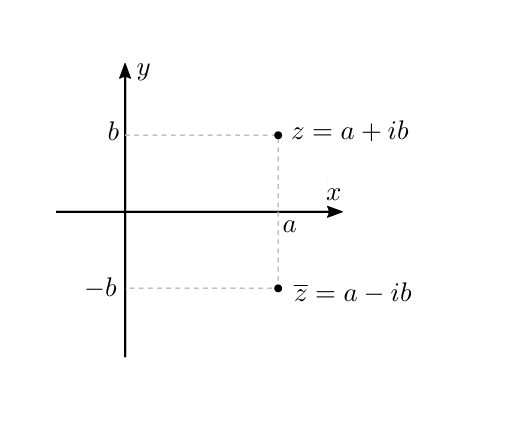
\includegraphics[width=0.5\textwidth]{Screenshot 2026-09-17 1656441.png}
		\caption{Geometrické znázornění komplexního čísla v rovině}
		\label{fig:my_image_2}
	\end{figure}
	
	Na obrázku 1.1 je kromě čísla $z = a+bi$ znázorněné také číslo komplexně sdružené k $z$, tj. číslo $\overline{z} = a - bi$. Geometricky je komplexně sdružené číslo $\overline{z}$ symetrické s číslem $z$ vzhledem k reálné ose.
	
	\medskip
	
	V geometrickém znázornění můžeme považovat komplexní číslo $z$ za polohový vektor. Toto poskytuje geometrickou interpretaci základních algebraických operací, jakožto sčítání a odčítání komplexních čísel.
	
	\begin{figure}[htbp]
		\centering
		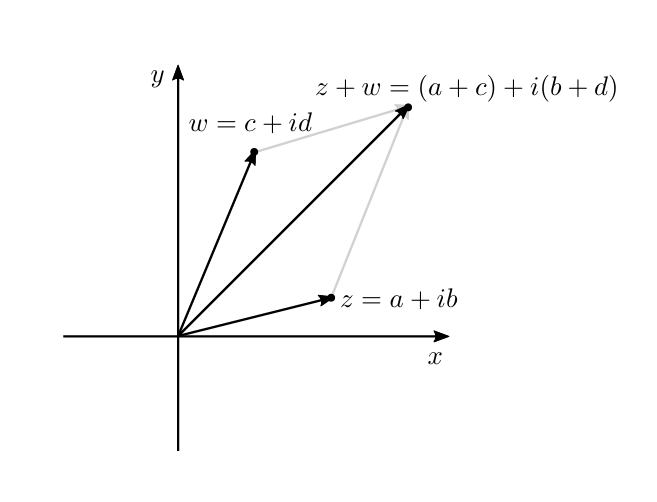
\includegraphics[width=0.5\textwidth]{Screenshot 2026-09-17 165941.png}
		\caption{Součet komplexních čísel}
		\label{fig:my_image_3}
	\end{figure}
	
	
	\section{Polární souřadnice v rovině}
	
	Geometrický význam násobení komplexních čísel je o něco složitější. Pro jeho pochopení je vhodnější použít k zápisu bodů v rovině polární souřadnice. V rovině s kartézskými souřadnicemi můžeme každý bod $P = (a,b)$ různý od počátku souřadnic jednoznačně určit pomocí vzdálenosti $r > 0$ bodu $P$ od počátku a orientovaného úhlu $\alpha$, který dostaneme tak, že kladnou $x_1$-ovou poloosu otáčíme kolem počátku souřadnic proti směru hodinových ručiček až do polopřímky s počátkem v bodě $(0,0)$ procházející bodem $P$. Dvojici čísel $(r, \alpha)$ nazýváme polární souřadnice bodu $P$, viz. obrázek 1.3. Protože otočením o plný úhel $2\pi$ neboli $360$ stupňů dostaneme zpět kladnou poloosu $x_1$, není úhel $\alpha$ určený jednoznačně. Různé možné hodnoty $\alpha$ se liší o nějaký celočíselný násobek $2\pi$. V případě, že $P = (0,0)$ je počátek souřadnic, je $r = 0$ a úhel $\alpha$ není definován.
	
	\begin{figure}[htbp]
		\centering
		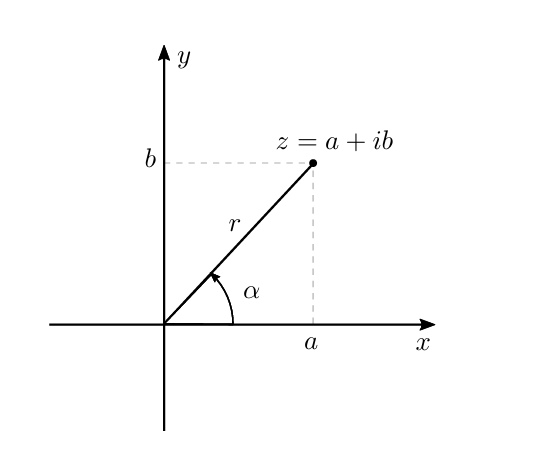
\includegraphics[width=0.5\textwidth]{Screenshot 2026-09-17 171211.png}
		\caption{Polární souřadnice bodu v rovině}
		\label{fig:my_image_4}
	\end{figure}
	
	Z polárních souřadnic $(r,\alpha)$ bodu $P \neq (0,0)$ vypočteme jeho kartézské souřadnice $(a,b)$ jako $a = r\cos\alpha$, $b = r\sin\alpha$.
	
	Naopak z kartézských souřadnic $(a,b)$ bodu $P \neq (0,0)$ dostaneme jeho polární souřadnice pomocí vztahů
	
	\begin{equation}
		r = \sqrt{a^2+b^2},\, \cos\alpha = \frac{a}{\sqrt{a^2+b^2}},\, \sin\alpha = \frac{b}{\sqrt{a^2+b^2}}.
	\end{equation}
	
	Protože funkce sinus a kosinus mají periodu $2\pi$, plyne odtud znovu, že úhel $\alpha$ je určený jednoznačně až na celočíselný násobek $2\pi$.

	\newpage
	
	\section{Goniometrický tvar komplexního čísla}
	
	Bod $P$ odpovídá komplexnímu číslu $z = a+bi$. Vyjádříme-li jeho kartézské souřadnice $(a,b)$ pomocí polárních, dostaneme
	
	\begin{equation}
		z = a+bi = r\cos\alpha + r\sin\alpha\cdot i = r(\cos\alpha + \sin\alpha\cdot i).
	\end{equation}
	
	Vyjádření $z = r(\cos\alpha + \sin\alpha\cdot i)$ nazýváme \textit{goniometrický tvar} komplexního čísla $z \neq 0$.
	
	\begin{itemize}
		\item číslo $r$ nazýváme \textit{absolutní hodnota} čísla $z$ a označujeme jej $|z|$,
		\item úhel $\alpha$ nazýváme \textit{argument} komplexního čísla $z$ a označujeme jej $\arg z$.
	\end{itemize}
	
	Platí tedy
	
	\begin{equation}
		|z| = \sqrt{a^2+b^2},\, \cos(\arg z) = \frac{a}{\sqrt{a^2+b^2}},\, \sin(\arg z)=\frac{b}{\sqrt{a^2+b^2}},
	\end{equation}
	
	také $\arg z$ může nabývat různých hodnot, které se ale vždy liší o celočíselný násobek $2\pi$. Protože platí, že $z\overline{z} = a^2 + b^2$, dostáváme pro absolutní hodnotu čísla $z$ vyjádření
	
	\begin{itemize}
		\item $|z|^2 = z\overline{z}$.
	\end{itemize}
	
	
	\section{Geometrický význam násobení komplexních čísel}
	
	Body na jednotkové kružnici odpovídají komplexním číslům $\cos\alpha + \sin\alpha\cdot i$. Takovým číslům říkáme komplexní jednotky. Pro součin dvou komplexních jednotek $w = \cos\alpha + \sin\alpha\cdot i$ a $z = \cos\beta + \sin\beta\cdot i$ platí
	
	\begin{align}
		&wz = (\cos\alpha + \sin\alpha\cdot i)(\cos\beta + \sin\beta\cdot i)\\
		&\phantom{wz} = \cos\alpha\cos\beta-\sin\alpha\sin\beta + (\cos\alpha\sin\beta + \sin\alpha\cos\beta)i\\
		&\phantom{wz} = \cos(\alpha + \beta) + \sin(\alpha + \beta)i
	\end{align}
	
	
	v poslední rovnosti jsme použili vzorce pro sinus a kosinus součtu dvou úhlů.
	
	\begin{figure}[htbp]
		\centering
		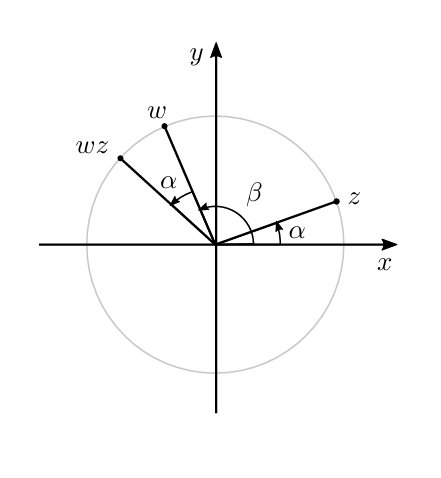
\includegraphics[width=0.5\textwidth]{Screenshot 2026-09-17 194335.png}
		\caption{Součin komplexních jednotek}
		\label{fig:my_image_5}
	\end{figure}
	
	\newpage
	
	Součin dvou komplexních jednotek je tedy opět komplexní jednotka, pro kterou platí
	
	\begin{equation}
		\arg(wz) = \arg w + \arg z,
	\end{equation}
	
	rovnost platí až na celočíselný násobek $2\pi$. Jednoduchou indukcí podle $n$ pak snadno dokážeme důležitou Moivreovu větu:
	
	\textit{Pro každý úhel $\alpha$ a každé přirozené číslo $n$ platí}
	
	\begin{equation}
		(\cos\alpha+\sin\alpha\cdot i)^n = \cos(n\alpha) + \sin(0\alpha)i.
	\end{equation}
	
	Důkaz. Pro $n = 0$ Moivreova věta zjevně platí, neboť
	
	\begin{equation}
		(\cos\alpha+\sin\alpha\cdot i)^0 = 1 = \cos 0 = \cos(0\alpha) + \sin(0\alpha)i.
	\end{equation}
	
	Předpokládejme, že platí
	
	\begin{equation}
		(\cos\alpha+\sin\alpha\cdot i)^n = \cos(n\alpha) + \sin(0\alpha)i.
	\end{equation}
	
	pro nějaké přirozené $n \ge 0$. Z tohoto indukčního předpokladu a součtových vzorců pro \textit{sinus} a \textit{kosinus} pak spočítáme, že
	
	\begin{align}
		(\cos\alpha + \sin\alpha\cdot i)^{n+1}&= (\cos\alpha + \sin\alpha\cdot i)^n(\cos\alpha + \sin\alpha\cdot i) =\\
		&= (\cos(n\alpha) + \sin(n\alpha)\cdot i)(\cos\alpha + \sin\alpha\cdot i) =\\
		&= (\cos(n\alpha)\cos\alpha - \sin(n\alpha)\sin\alpha)+(\cos(n\alpha)\sin\alpha + \sin(n\alpha)\cos\alpha)\cdot i =\\
		&= \cos[(n+1)\alpha] + sin[(n+1)\alpha]\cdot i,
	\end{align}
	
	čímž je indukční krok dokázán. \hfill$QED$
	
	\medskip
	
	Jsou-li nyní $w = r(\cos\alpha + \sin\alpha\cdot i)$ a $z = s(\cos\beta + \sin\beta\cdot i)$ libovolná dvě nenulová komplexní čísla, pak pro jejich součin platí
	
	\begin{align}
		&wz = r(\cos\alpha + \sin\alpha\cdot i)s(\cos\beta + \sin\beta\cdot i)\\
		&\phantom{wz} = rs(\cos\alpha + \sin\alpha\cdot i)(\cos\beta + \sin\beta\cdot i)\\
		&\phantom{wz} = rs(\cos(\alpha + \beta) + \sin(\alpha + \beta)\cdot i).
	\end{align}
	
	Pro absolutní hodnotu a argument součinu $wz$ tak platí
	
	\begin{itemize}
		\item $|wz| = |w||z|,$
		\item $\arg(wz) = \arg w + \arg z.$
	\end{itemize}
	
	\begin{figure}[htbp]
		\centering
		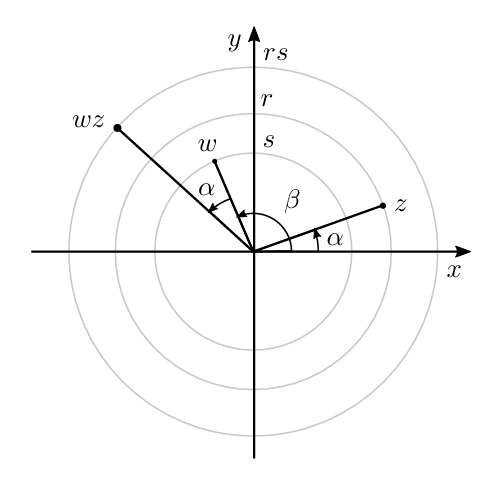
\includegraphics[width=0.5\textwidth]{Screenshot 2026-09-17 203534.png}
		\caption{Součin komplexních čísel}
		\label{fig:my_image_6}
	\end{figure}
	
	\newpage
	
	V jednoduchém speciálním případě, kdy $w = i = \cos(\frac{\pi}{2}) + \sin(\frac{\pi}{2})\cdot i$ dostáváme, že $|zi| = |z||i| = |z|$ a $\arg(zi) = \arg z + \arg i = \frac{\pi}{2} + \arg z$. Vynásobit číslo $z$ číslem $i$ tak znamená pootočit číslo $z$ kolem počátku souřadnic o pravý úhel proti směru hodinových ručiček. To můžeme také snadno nahlédnout z algebraického tvaru $z = a + bi$, neboť $zi = (a+bi)i = -b + ai$.
	
	\begin{figure}[htbp]
		\centering
		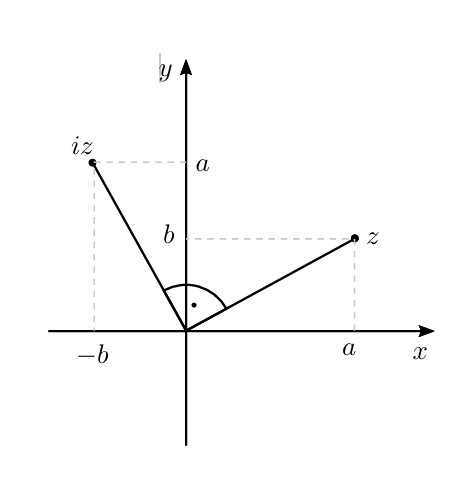
\includegraphics[width=0.5\textwidth]{Screenshot 2026-09-17 204153.png}
		\caption{Součin komplexního čísla s imaginární jednotkou}
		\label{fig:my_image_7}
	\end{figure}
	
	\newpage
	
	\section{Komplexní exponenciála}
	
	
	\textit{Komplexní exponenciálu} definujeme pomocí Eulerovy formule
	
	\begin{equation}
		e^{i\alpha} = \cos\alpha + \sin\alpha\cdot i.
	\end{equation}
	
	pro každé reálné číslo $\alpha$. Speciálním případem je elegantní \textit{Eulerova identita}
	
	\begin{equation}
		e^{i\pi} = -1.
	\end{equation}
	
	Eulerovu formuli lze použít jako pohodlnější zápis komplexních jednotek $\cos\alpha + \sin\alpha\cdot i$. Dříve dokázané vlastnosti součinu dvou komplexních čísel můžeme pomocí Eulerovy formule zapsat jako pravidla pro počítání s mocninami, které v případě reálných exponentů znáte ze střední školy. Vzorec pro součin dvou komplexních jednotek pak můžeme zapsat jako
	
	\begin{equation}
		e^{i\alpha}e^{i\beta} = e^{i(\alpha+\beta)}.
	\end{equation}
	
	Podobně jednoduše lze zapsat Moivreovu větu:
	
	\begin{equation}
		(e^{i\alpha})^n = e^{i(n\alpha)}.
	\end{equation}
	
	Goniometrický tvar nenulového čísla $w = r(\cos\alpha + \sin\alpha\cdot i)$ je potom
	
	\begin{equation}
		z = re^{i\alpha} = e^{\ln r + \alpha\cdot i},
	\end{equation}
	
	kde $r = |w|$ a $\alpha = \arg w.$
	
	
	\section{Trojůhelníková nerovnost}
	
	Dokážeme si ještě dvěma způsoby trojúhelníkovou nerovnost pro komplexní čísla, která říká, že pro libovolná dvě čísla $z = a+bi$ a $w = c+di$ platí
	
	\begin{itemize}
		\item $|w+z| \le |w| + |z|.$
	\end{itemize}
	
	K algebraickému důkazu trojúhelníkové nerovnosti využijeme další dvě jednoduché vlastnosti absolutní hodnoty komplexních čísel. Pro každé komplexní číslo $z = a+bi$ platí
	
	\begin{itemize}
		\item $|z| = |\overline{z}|,$
		\item $\text{Re}z \le |z|.$
	\end{itemize}
	
	První rovnost plyne přímo z definice absolutní hodnoty, dokážeme druhou. Je-li $z =a+bi$, pak platí
	
	\begin{equation}
		a\le |a| = \sqrt{a^2} \le \sqrt{a^2 + b^2} = |z|.
	\end{equation}
	
	\newpage
	
	Pro každou rovnost nebo nerovnost v následujícím výpočtu (s výjimkou poslední rovnosti) si najděte v předchozím textu tu vlastnost komplexních čísel, kterou používáme.
	
	
	\begin{align}
		|z + w|^2 &= (z + w)(\overline{z + w}) = (z + w)(\overline{z} + \overline{w}) = z\overline{z} + z\overline{w} + w\overline{z} + w\overline{w}\\
		&= |z|^2 + z\overline{w} + w\overline{z} + |w|^2 = |z|^2 + z\overline{w} + \overline{z\overline{w}} + |w|^2\\
		&= |z|^2 + 2\,\text{Re}\,(z\overline{w}) + |w|^2 \le |z|^2 + 2z\overline{w} + |w|^2 = |z|^2 + 2|z||\overline{w}| + |w|^2\\
		&= |z|^2 + 2|z||w| + |w|^2 = (|z| + |w|)^2.
	\end{align}
	
	Dokázali jsme tak $|z + w|^2\le(|z| + |w|)^2$ a po odmocnění dostáváme trojúhelníkovou nerovnost pro komplexní čísla. Pomocí geometrického významu sčítání komplexních čísel trojúhelníkovou nerovnost snadno nahlédneme z obrázku.
	
		\begin{figure}[htbp]
		\centering
		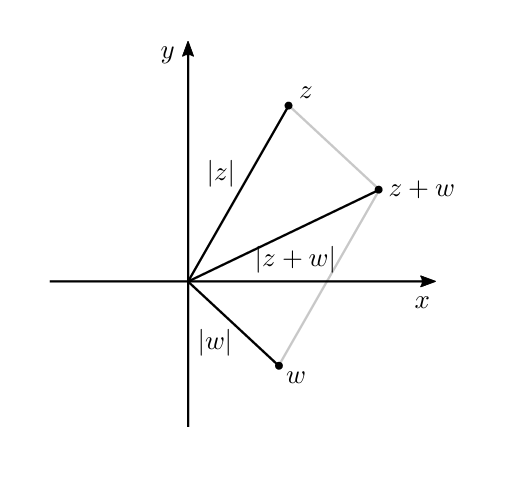
\includegraphics[width=0.5\textwidth]{Screenshot 2026-09-18 205004.png}
		\caption{Trojúhelníková nerovnost pro komplexní čísla}
		\label{fig:my_image_8}
	\end{figure}
	
	\newpage
	
	\section{Úlohy -- komplexní čísla}
	
	
	
	
	
	
\end{document}